\documentclass[a4paper,12pt]{article}
\usepackage[T2A]{fontenc}
\usepackage[utf8]{inputenc}
\usepackage[english,russian]{babel}
\usepackage[pdftex,unicode]{hyperref}
\usepackage[pdftex]{graphicx}
\usepackage{float}
\graphicspath{{graphicx/}}
\DeclareGraphicsExtensions{.pdf,.png,.jpg}
\usepackage{indentfirst}
\usepackage[left=2cm,right=2cm,
    top=2cm,bottom=2cm,bindingoffset=0cm]{geometry}

\begin{document}
	\begin{center}
		\section{ Длинная динамика для мез 600/100 и 1200/100.}
	\end{center}
	\subsection{Уравнение аппроксимации}
	Аппроксимировал данные с помощью следующего уравнения:
	\begin{equation}
		fit(t) = (1-A_0)\left(1-a e^{- \left(\frac{t - t_o}{c}\right)} - (1-a)e^{- \left(\frac{t - t_o}{d}\right)}\right) + A_0
	\end{equation}
	где $a$, $c$ и $d$ коэффициенты аппроксимации,\\
	$t_0$ - момент времени, выбранный для начала аппроксимации\\
	$A_0$ - амплитуда, в начальный момент времени.
	\subsection{Результаты для мезы 600/100}
		\begin{figure}[H]
			\center{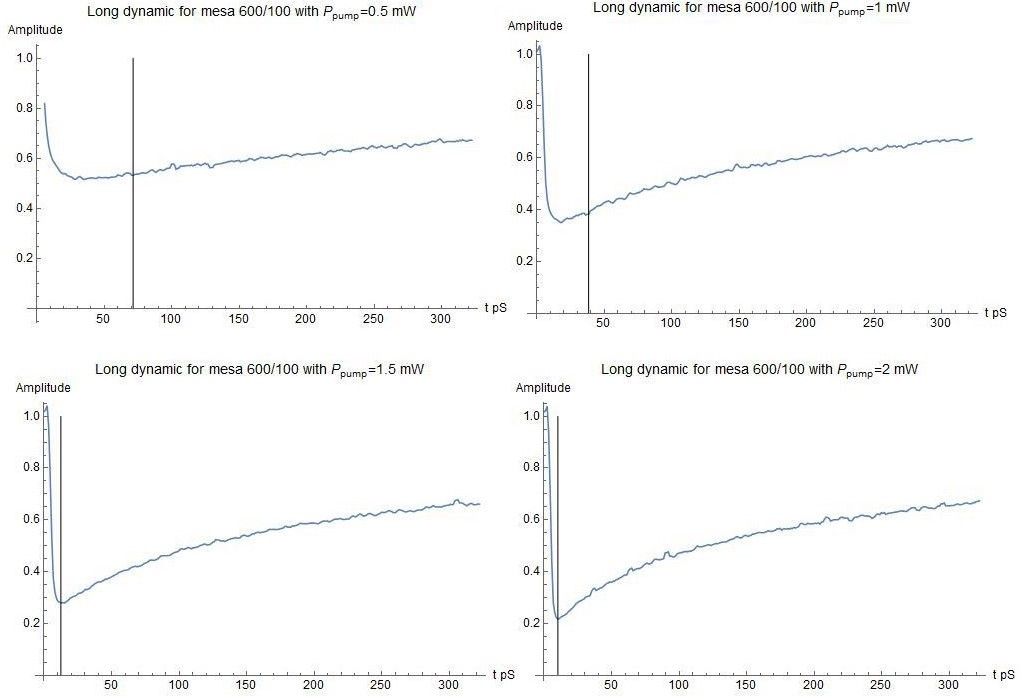
\includegraphics[scale=0.48]{long600100}}
			\caption{Выбор начала аппроксимации}
		\end{figure}
		\begin{figure}[H]
			\center{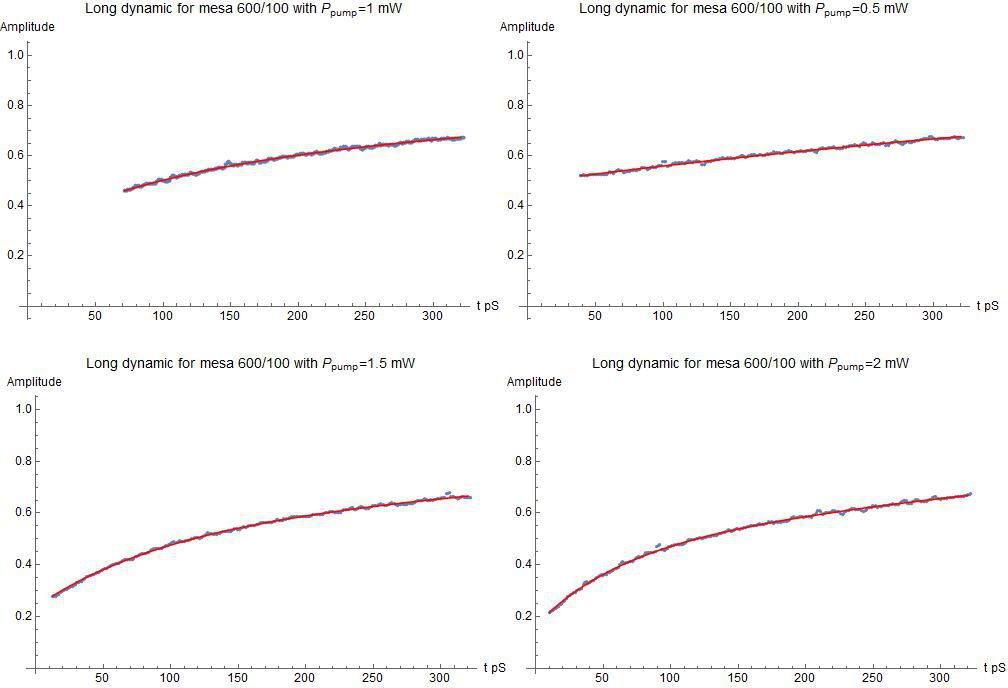
\includegraphics[scale=0.48]{apLong600100}}
			\caption{Результат аппроксимации}
		\end{figure}
		\begin{figure}[H]
			\center{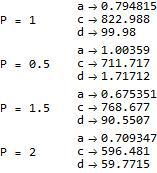
\includegraphics[scale=0.8]{table600100}}
			\caption{Найденные параметры}
		\end{figure}	
\newpage
	\subsection{Результаты для мезы 1200/100}
		\begin{figure}[H]
			\center{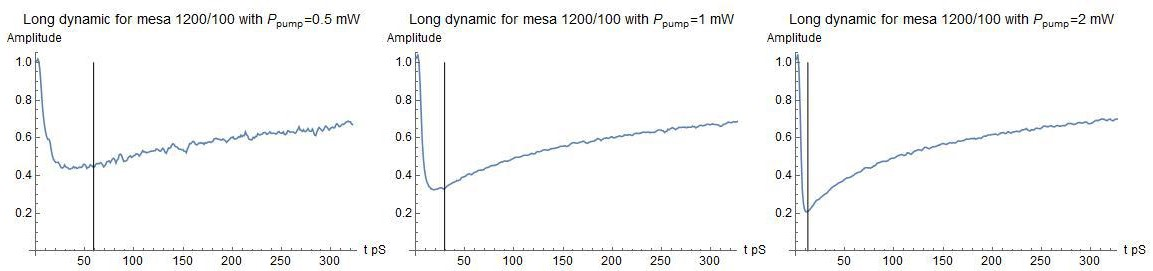
\includegraphics[scale=0.4]{long1200100}}
			\caption{Выбор начала аппроксимации}
		\end{figure}
		\begin{figure}[H]
			\center{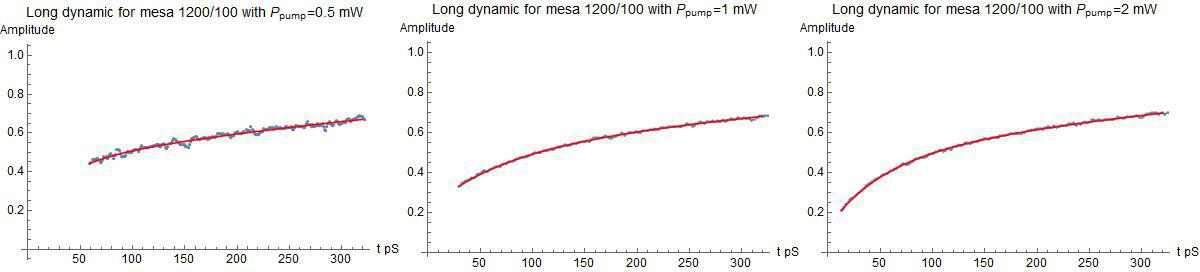
\includegraphics[scale=0.4]{apLong1200100}}
			\caption{Результат аппроксимации}
		\end{figure}
		\begin{figure}[H]
			\center{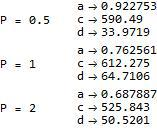
\includegraphics[scale=0.8]{table1200100}}
			\caption{Найденные параметры}
		\end{figure}
\newpage
	\subsection{Сравнение временных характеристик для мез 600/100 и 1200/100}
		\begin{figure}[H]
			\center{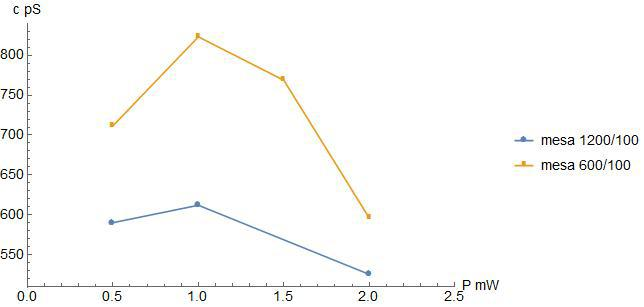
\includegraphics[scale=0.6]{longTime}}
			\caption{Зависимость "долгого" времени от мощности накачки}
		\end{figure}
		\begin{figure}[H]
			\center{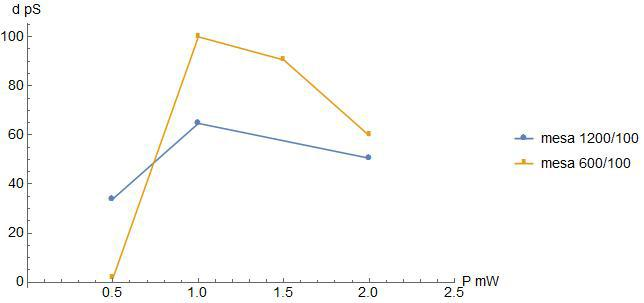
\includegraphics[scale=0.6]{shortTime}}
			\caption{Зависимость "быстрого" времени от мощности накачки}
		\end{figure}
\end{document}